\documentclass[11pt]{article}

\usepackage[margin=1in]{geometry}
\usepackage[T1]{fontenc}
\usepackage[utf8]{inputenc}
\usepackage{lmodern}
\usepackage{hyperref}
\usepackage{pdfpages}

\hypersetup{
  pdftitle={The Construction of Living Robots: LaTeX Facsimile Edition},
  pdfauthor={Edmund C. Berkeley; facsimile edition prepared in repository},
  pdfsubject={Facsimile edition of a 1952 Berkeley robotics source},
  pdfkeywords={Edmund C. Berkeley, robotics, facsimile, living robots, symbolic logic}
}

\title{The Construction of Living Robots\\\large LaTeX Facsimile Edition}
\author{Original work by Edmund C. Berkeley}
\date{Original publication: 1952\\Facsimile edition prepared: August 5, 2026}

\begin{document}

\maketitle

\section*{Editorial Note}

This document is a modern LaTeX facsimile edition of Edmund C. Berkeley's
\emph{The Construction of Living Robots} (1952). It is included here because
the source is directly relevant to the repository's Berkeley--Heiserman paper
project.

The present edition is not yet a full diplomatic transcription. The source PDF
available in this repository is image-only, and local OCR tooling was not
available at preparation time. To preserve accuracy, the original scanned pages
are therefore reproduced intact inside a LaTeX wrapper rather than retyped by
hand.

\section*{Source}

Repository source file:

\begin{itemize}
\item \texttt{sources/Berkeley--The Construction of Living Robots.pdf}
\end{itemize}

\clearpage

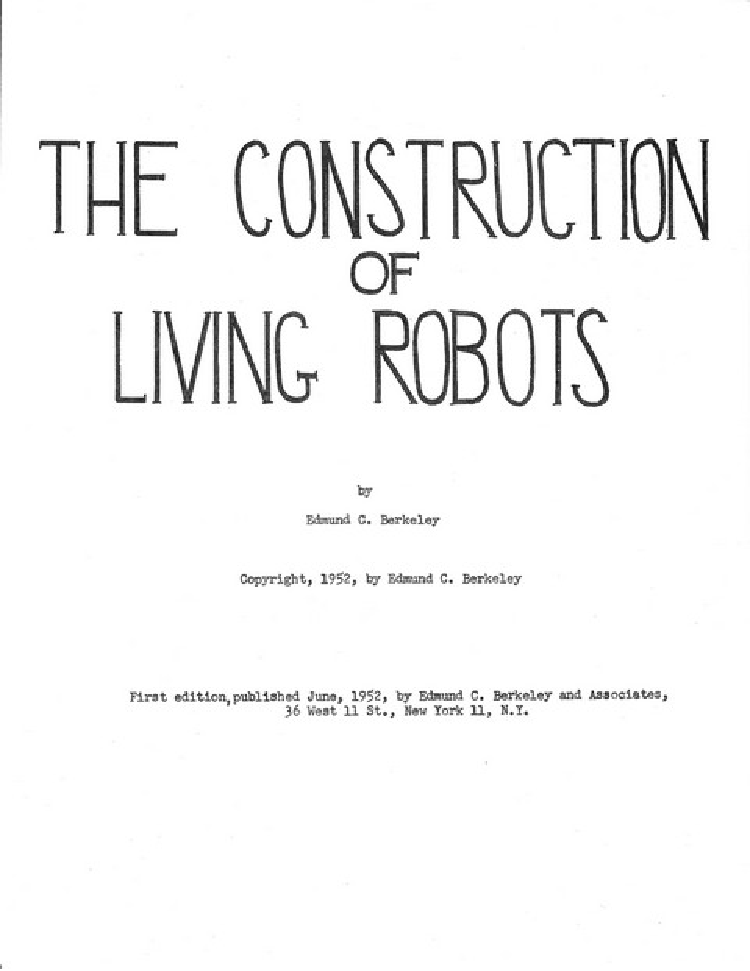
\includepdf[pages=-]{../../sources/Berkeley--The Construction of Living Robots.pdf}

\end{document}
